\subsection{Scrum Revisited}
We will revisit Scrum one final time, and discuss the Scrum Retrospective and Scrum Review.
\subsubsection{Scrum Review}
At this point, the final sprint has come to an end, and we review what we have gotten done in this sprint. Normally we would review each story on the backlog and possibly make changes, but since this is the final sprint, it is too late to change anything.\\
\newline
\begin{figure}[H]
  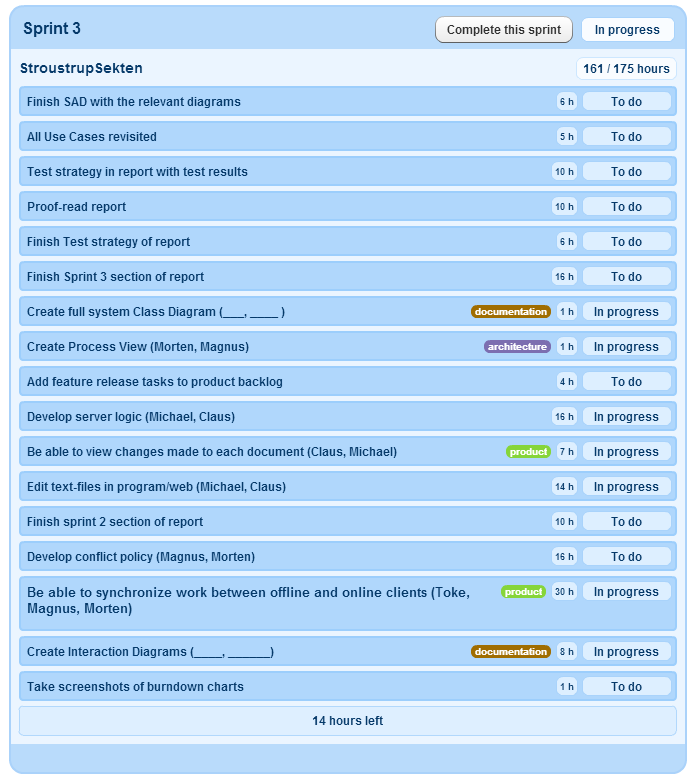
\includegraphics[width=\textwidth]{illustrations/sprint3backlog.PNG}
  \caption{Sprint 3 Backlog}
  \label{sprint3backlog}
\end{figure}
\textbf{Meeting summary}\\
The planned stories for the sprint was finished within the time limits. Most importantly, we meet all requirements and the hand-in deadline was met.\\
The structure of the program seems solid, flexible and easy to maintain. In this sprint, we have added functionality to the GUI's such as Changes and Sharing of documents. This was very easy to do, with the back-end structure we have carefully designed and implemented.\\
\newline
No changes to the backlog is made, but a few stories remain, for optional future implementation. See [Appendix ref or add fig]
\begin{figure}[H]
  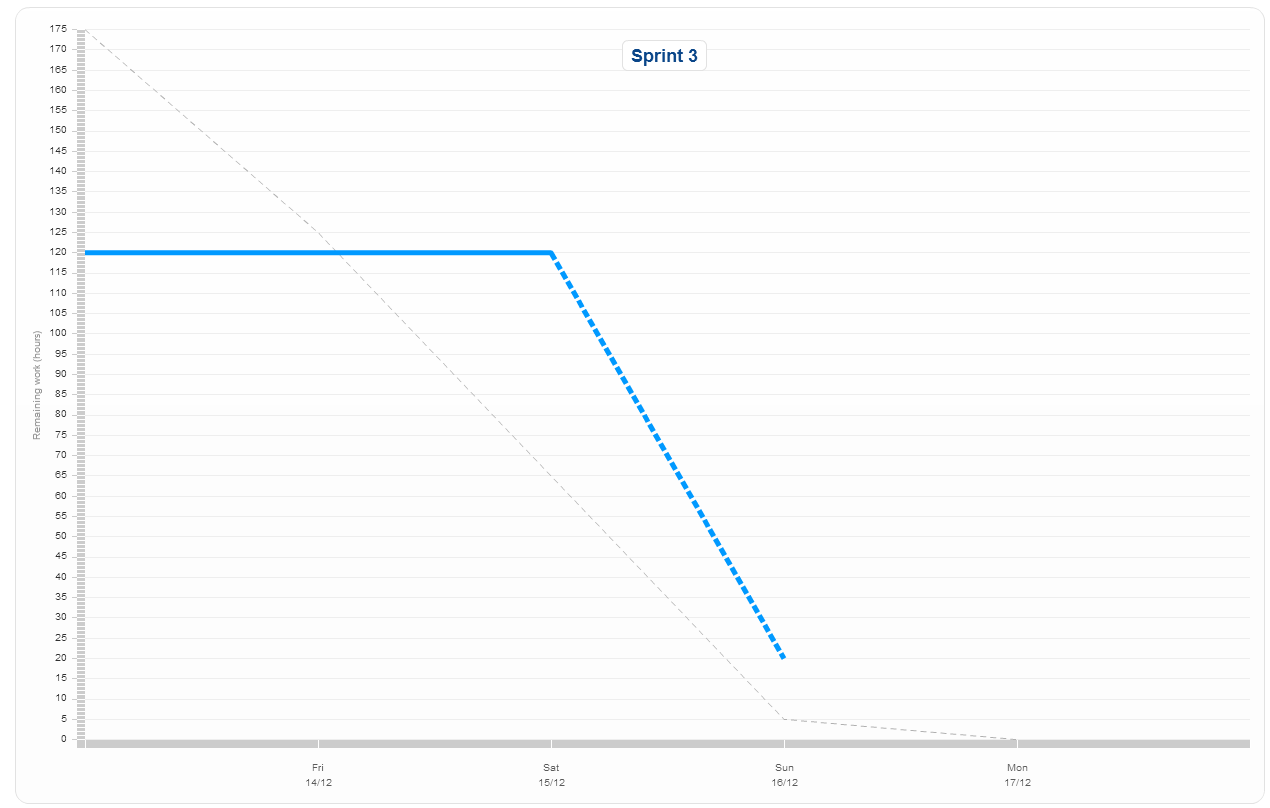
\includegraphics[width=\textwidth]{illustrations/sprint3burn.PNG}
  \caption{Sprint 3 Burnchart}
  \label{sprint3burnchart}
\end{figure}
\subsubsection{Scrum Retrospective}
It was a short sprint of only three days, and it went well.\\
\newline
\textbf{Improvements}
The Scrum Team has no further improvement suggestions at this time.\\